\title{ 8-bit Parallel-In/Serial-Out shift register}
\date{2024-08-31}
\author{
	\IEEEauthorblockN{Daniel Josué Rodríguez Agraz}
	\IEEEauthorblockA{
		\textit{Ingeniería en Electrónica y Comunicaciones, Unniversidad de Guadalajara}
	}
}

\documentclass[9pt,technote]{IEEEtran}
\usepackage[noadjust]{cite}
\usepackage{graphicx}
\usepackage{footmisc}
\usepackage{listings}
\usepackage{subcaption}
\usepackage{fancyhdr}
\usepackage{url}
\usepackage{amsmath}
\usepackage{hyperref}
\usepackage{array}
\usepackage{float}



\begin{document}
	
	\maketitle
	\section{Objectives}
	\begin{itemize}
		\item Use Verilog to design and simulate an 8-bit Parallel-In/Serial-Out shift register using the IC 74HC165 specifications.
		\item Design a test bench for the circuit verification.
	\end{itemize}
	
	\section{Introduction} 
	A register is a digital circuit with two main functions: data storage and data movement. The storage characteristic of a register refers to the total number of bits of digital data it can hold. The shifting characteristic allows data to flow from one stage to another within the register or to its input or output, depending on the clock pulses applied.\cite{floyd_fundamentos_nodate}
	
	The figure \ref{} shows the symbol of an 8-bit parallel-in/serial-out shift register.

	\begin{figure}[H]
		\centering
		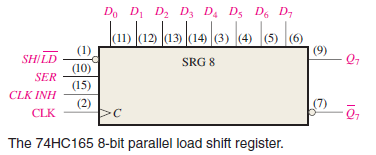
\includegraphics[width=0.8\columnwidth]{Diagrama}
		\caption{Symbol of an 8-bit shift register.}
		\label{fig:diagrama}
	\end{figure}
	

	A register is created by combining flip-flops to store and shift data (1's and 0's) and typically does not possess an internal state sequence.

	There are two main types of registers: serial and parallel. In a serial shift register, bits are stored sequentially, as shown in Figure \ref{fig:serialserialreg}. The most significant bit (MSB) of the input signal is placed in the least significant bit (LSB) position of the register, and the rest of the bits are shifted to the right. The output is the value of the most significant bit. of the register.\cite{floyd_fundamentos_nodate}
	
	\begin{figure}[H]
		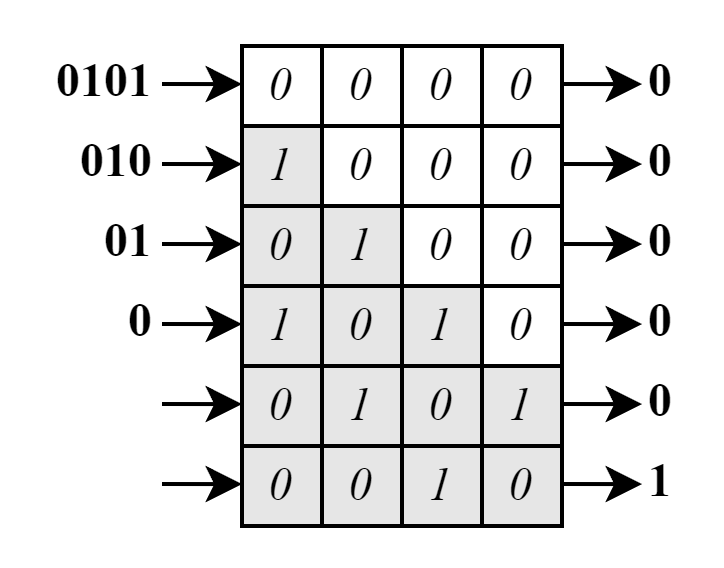
\includegraphics[width=0.7\columnwidth]{serial_serial_reg}
		\caption{Example of a 4-bit shift serial register, where each cell represents a flip-flop.}
		\label{fig:serialserialreg}
	\end{figure}

	In a parallel register, bits are stored simultaneously from parallel lines, as illustrated in Figure \ref{fig:parallelserialreg}.
	
	\begin{figure}[H]
		\centering
		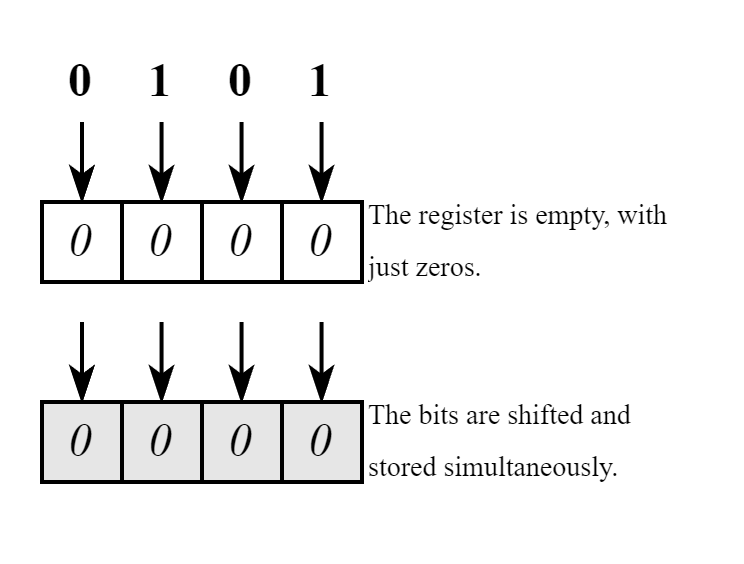
\includegraphics[width=0.7\columnwidth]{Parallel_serial_reg}
		\caption{Example of a 4-bit shift parallel register, where each cell represents a flip-flop.}
		\label{fig:parallelserialreg}
	\end{figure}
	
	
	
	
	
	\section{Methodology}
	The 8-bit Parallel-In/Serial-Out shift register has been developed in two stages. In the first step the register has been designed based on the IC 74HC165 specifications available in the literature \cite{texas_instruments_sn74hc165}. Using the truth table and the sequence diagram provided by the datasheet, shown in the Table \ref{table:function-table}, extracted from the page 13th.
	
	\begin{table}[H]
		\centering
		\includegraphics[width=\columnwidth]{"Function table"}
		\caption{Input signals function table for the shift register SN74HC165.}
		\label{table:function-table}
	\end{table}
	
	As the datasheet mentions on page 1, the CLK and CLKINH pins are interchangeable, because low CLK and a low-to-high transition of CLK INH also accomplish clocking, CLK INH must be changed to the high level only while CLK is high. Parallel loading is inhibited when SH/LD is held high. While SH/LD is low, the parallel inputs to the register are enabled independently of the levels of the CLK, CLK INH, or serial (SER) inputs.\cite{texas_instruments_sn74hc165}
	
	\begin{figure}[H]
		\centering
		\includegraphics[width=0.9\columnwidth]{"Logic diagram"}
		\caption{Logic diagram for the shift register SN74HC165.}
		\label{fig:logic-diagram}
	\end{figure}
	
	To develop the register, I referenced the diagrams provided in the datasheet on page 1, Figure \ref{fig:logic-diagram}. I considered that CLK and CLKINH (which is referred to as $clken$ in the code) are ORed, and implemented this logic directly in the code, as shown below.
	
	\begin{lstlisting}[language=Verilog, caption={Verilog code for an 8 bit shift register.}, label={code:audio_correlation}]
	module PISO_REG_4B(
	input reg[0:7] D_in,
	input reg LOAD, SER,
	input reg clk, clken,
	output reg Q, QNEG
	);
	
	reg [0:7] D;
	assign QNEG = ~Q;
	assign Q = D[7];
	
	always@(posedge clk or posedge clken)
	begin
	if (~LOAD)
	begin
	  D <= D_in;
	end 
	else if (~clk | ~clken)
	begin
	  D <= D >> 1;
	  D[0]<=SER;
	end
	end
	endmodule
	\end{lstlisting}
	
	\section{Results}
		
	For the test bench all the input pins were initialized as shown in the Table \ref{table:Init table}. It can be noticed from the truth table \ref{table:function-table}, when initialized either clk or clkinh (clken) in a high state, the value at the output is indefinite.
	
	\begin{table}
		\centering
		\begin{tabular}{|c|c|c|c|}
			\hline
			clk & clken & LOAD & ser \\
			\hline
			0 & 1 & 1 & 0 \\
			\hline
		\end{tabular}
		\caption{Initialization values.}
		\label{table:Init table}
	\end{table}
	
	We then loaded a value into the register by setting LOAD to high, and the output takes the value of the most significant bit of the data as shown on the Figure \ref{fig:timediagram} where the signal in the Figure \ref{fig:timediagram:1b} imitates the time diagram provided by the datasheet on page 12.
	
	\begin{figure}[H]
		\begin{subfigure}[b]{\columnwidth}
			\centering
			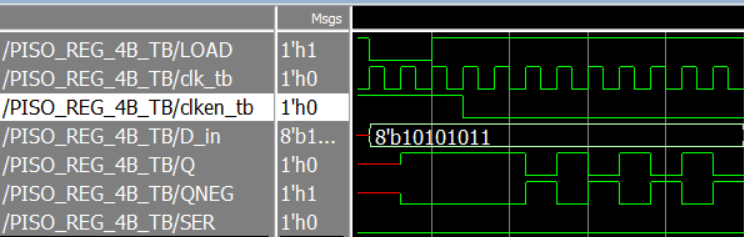
\includegraphics[width=0.9\columnwidth]{time_diagram1}
			\caption{Simulation results of the shift register (part 1).}
			\label{fig:timediagram:1b}
		\end{subfigure}
		\vspace{0.5cm}
		\begin{subfigure}[b]{\columnwidth}
			\centering
			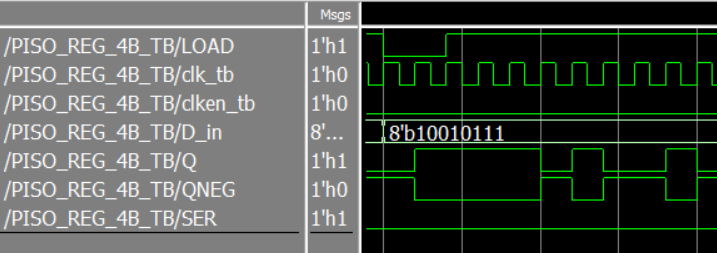
\includegraphics[width=0.9\columnwidth]{time_diagram2}
			\caption{Simulation results of the shift register (part 1).}
			\label{fig:timediagram:2b}
		\end{subfigure}
		\caption{Time diagram of the test bench.}
		\label{fig:timediagram}
	\end{figure}
	
	\begin{figure}[H]
		\centering
		\includegraphics[width=0.7\columnwidth]{"time_diagram datasheet"}
		\caption{Time diagram provided by the datasheet.\cite{}}
		\label{fig:timediagram-datasheet}
	\end{figure}
	
	Finally, to start the shifting process, the $clken$ signal was set to low. As shown in Figure \ref{fig:timediagram3}, when the pin is set to high again, the register stops shifting, and the output takes the value of the last internal most significant bit.
	
	\begin{figure}[H]
		\centering
		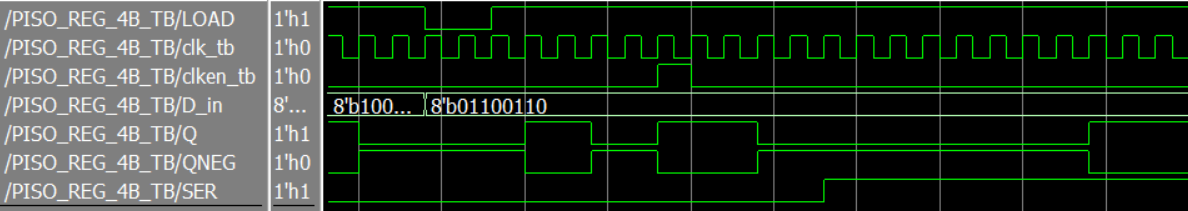
\includegraphics[width=\columnwidth]{time_diagram3}
		\caption{Simulation results of the shift register (part 3).}
		\label{fig:timediagram3}
	\end{figure}
	
	
	The serial pin replaces the most significant bit of the internal register until all the parallel data leaves the register, this allows us to put two of this registers together to create a 16-bit shift register.
	
	
	
	
	\section{Conclusiones}
	In this document, an 8-bit Parallel-In/Serial-Out shift register was designed and tested. The register, based on the IC 74HC165 specifications, produced the same results under identical inputs during the test bench evaluation. The test bench results indicate, that the designed register can be used as a commercial Parallel-In/Serial-Out shift register. 
	
	
	
	
	
	
	
	
	
	
	\bibliographystyle{IEEEtran}
	\bibliography{References}
	
	
	
	
	
	
	
	
\end{document}
